\section{Cryptography}
\subsection{Post-Quantum Cryptography}
\label{subsec:post-quantum_cryptography}
Post-Quantum Cryptography (PQC) describes ciphers which are designed to be post-quantum- era safe. This involves finding quantum-safe trapdoor functions\footnote{Computationally-efficient to compute `forwards', but, crucially, highly- computationally-expensive to compute backwards (e.g. decryption without correct keys, etc.)}. One way this is presently achieved is to base the trapdoor function off a computationally- expensive/hard problem, such as the learning-with-errors lattice problem, as in the case of CRYSTALS-Kyber (\cref{para:pqxdh}) \citep{wikipedia:kyber} -- instead of, for example, elliptic curves (using Shor's algorithm to efficiently back-calculate the private key from the public key, since ECC relies on the computational hardness of the discrete-logarithm problem).
\subsubsection{PQC in TLS}%TODO proof read; thisis goin in appendix i reckon
\label{subsubsec:pqc_in_tls}
Modern browsers are attempting integration of PQ key-exchange and PQ authentication methods into their cipher suites (presence advertised in their TLS-ClientHello packet, sent when negotiating a TLS-secured web connection), in order to prevent store-then-decrypt attacks (see \cref{subsubsec:the_signal_protocol}). However, due to a bug in present in some older (/poorly-developed) web servers, dubbed `tldr.fail', a ClientHello packet must be contained within 1 packet. This presents a problem for TLS-ClientHello packets which advertise support for PQ cryptographic methods, since such packets are larger than the accepted-maximum- size of a TCP packet's (segment) payload, which, in practice, for IPv4, is 1480 bytes, where typical MTU is 1500 bytes, and its IPv4 header occupies at minimum 20 bytes total (maximum payload size with 20b header is therefore 1480 bytes (with 1500b MTU), as above) however the header size varies, and can be as large as 80b, which (assuming the same standardised 1500b MTU) leaves only 1420b for the payload\footnote{Interestingly, however, variable header size is only applicable to IPv4; IPv6 has a \textbf{fixed} header size of 40 bytes, so with the same 1500b MTU (although with the use of MTU path discovery, the MTU may be increased if all en-route nodes support a higher MTU) the payload is always 1460b.}.\\
In theory, with large-scale adoption of (super-) jumbo frames\footnote{Super-jumbo frames can theoretically be as large as $(2^{16}-1 =) 65535$ bytes (64KiB), however this particularly-large frame is likely not necessary for ClientHello packets with post-quantum cryptography. Furthermore, specifically jumbo frames (i.e. not packets -- referring here to once the frames are discarded at the router, then the packet within is sent over The Internet) themselves do not solve this issue, given that the Maximum Transmission Unit (MTU) (maximum size of a frame (or packet when outside the local network)) is set by the network handling the frame (or packet, on The Internet), as such jumbo frames only solve this problem if the all networks from the end-device to the server-to-negotiate-PQ-TLS have their MTU set equal to or larger than the ClientHello (or, more broadly, frame/packet-being-sent's) size, and \textbf{not} only on the local network, else this would be chunked/fragmented anyway, however only for IPv4, since with IPv6, routers do not fragment packets above the MTU, rather it drops the packet (to discover the highest MTU to use, techniques such as MTU discovery can be employed to discover each router- en-route's MTU, then using the lowest MTU discovered, allowing packets to potentially be sent at a higher size (if MTUs en route allow such)).} (or similar) (and subsequent (super-) jumbo packets), the PQC ClientHello could fit in a single packet, however even so this may require changes to the web server itself, since if the web server is, again, poorly-developed such that it may explicitly read $X$ bytes, then will discard the rest of the ClientHello packet, or perhaps worse still if server is set to read the whole packet into a fixed-size buffer, the size of which is set to, e.g., the size of the maximum IPv4 payload (assuming standard MTU of 1500b) (potentially causing buffer overflow/segmentation-fault -- if it truly is \textit{that} poorly developed). _Furthermore, issues arise if MTUs Internet-wide increase because, as mentioned in the previous footnote, all nodes en-route to the destination need to also have the same (or larger MTU) -- in any event, increasing MTU to allow a larger ClientHello packet (thereby allowing ClientHello packet with PQC data to `fit' in one packet), still breaks if packet too large for old/poorly-developed web servers, due to aforementioned reasons.\\
Although, in the case of tldr.fail this is a result of the connection being reset by the web server after it receives a partial ClientHello packet -- and as explained above, increasing MTU does not strictly solve the problem since all routers require the increased MTU, else packets are chunked\footnote{Or dropped if `do not fragment' header option is set, or using IPv6 (dropped immediately; IPv6 packets cannot be chunked).}. Tldr.fail is problematic, since given a 1500b MTU, browsers could otherwise just send the larger ClientHello packet (with PQC data) chunked, e.g., ClientHello sent in 2 halves, but only if the web server does not reset the connection after receiving the first half of the ClientHello packet (as some older web servers appear to do, as outlined in this bug). If the web server resets the connection after receiving the first half of the ClientHello packet, when the server receives the 2nd half, it will see only the second half \textbf{not} in relation to the first, i.e. perceived random data, as such the PQC-TLS connection does not get established -- this is one of the problems web browsers are presently facing, since if they send the larger ClientHello packet with PQ-cipher- data, then they must send it in more than one packet, but if doing this for connections to all web servers, because of the tldr.fail bug being present in some web servers (preventing connection)\footnote{It appears to presently impossible to know ahead-of-time if the web server is prone to this bug, unless perhaps a list of such affected websites is maintained, and for sites on this list, the browser does not attempt to negotiate PQ ciphers, and disseminate this list to browsers -- or perhaps this is solvable by reducing the amount of data required for PQC in only the ClientHello packet, such that ClientHello packet is sent wholly , then the web server can query the client to determine if the client can support PQ ciphers. However, it may be such that all clients connecting to such a web server do not support PQC -- for these clients, the server could perhaps read the client's user agent to determine browser version; if browser version on list of supported clients, then server can query client for such PQ data -- this works as the client has a user agent, however the server does not have a similar way to advertise PQ-cipher support (in which case, the server could otherwise advertise such support, or advertise it not being prone to the tldr.fail bug, via some other method/band(-of-communication)).}.
%TODO mv. explanation of store-then-decrypt from subsubsec:theSignalProtocol to here. `store-then-decrypt' attacks (as referenced in \cref{subsubsec:pqc_in_tls})'
\subsubsection{The Signal Protocol}
\label{subsubsec:the_signal_protocol}
The Signal Protocol has various components incorporating Post-Quantum (PQ) encryption, as of August 2025 this protocol (and its double ratchet algorithm) is used in the latest version of the Signal messenger and WhatsApp, even though stable quantum computers are presently though to be theoretical-only, implementing and using PQ encryption now (before quantum era) is necessary to prevent `store-then-decrypt' attacks, which intercept and store encrypted messages now -- then assuming such stable quantum computers exist in the future, decrypt the stored messages at the point they exist (in a powerful-enough and robust fashion to break such encryption, which is presently thought to be safe/computationally-intractable for binary-classical (i.e. present computers; not quantum) computers).%TODO reread/reword this intro. + FACT CHECK IF PQC ACTUALLY USED IN SIGNAL + WHATSAPP
\paragraph{Diffie-Hellman Primer}
\label{para:diffie-hellman_primer}
\noindent\\
As simply-stated as possible, Diffie-Hellman (DH), in a 2-party transaction, involves each party generating a private and corresponding public key, then sending their public key to each-other, then each party combining (see below) the other's public key with their own private key, at which point both arrive at a shared-key (same key held by both).\\
More specifically, however, the key-generation is achieved by each party publicly sharing parameters of key-generation ahead-of-time, parameters such as a large-prime, $P$, and a generator, $G$, which must be a primitive-root of $P$. Furthermore, each must choose a private key, $A$ (Alice's private key), $B$ (Bob's private key), where, for example, $A$ is some random value less than $P$, but greater than 0 \citep{geeks:dh}.\\
If $G$ is \textbf{not} a primitive-root of $P$, upon calculating a public key via $G^A mod P$, the maximum number of non-repeating public keys (for a given private key) is not $P-1$, as such the search-space (number of \textbf{unique} combinations of possible public keys (from the private key)) is greatly-reduced. In contrast, if $G$ is a primitive-root of $P$, the maximum number of unique private keys is $P-1$ (larger search-space, therefore stronger).\\
As afore-explained, Alice therefore generates her public key with $G^A mod P$, and Bob generates his public key with $G^B mod P$, where $B$ is, again, a random value, also in the range 1..$P-1$ (but ideally also is a different value from $A$, since instead of having to calculate both $A$ and $B$, since they are equal, only one need-be found, however attempting to back-calculate each still relies on the hardness of the discrete-logarithm problem (resorting to brute-force, in effect), however there have been optimisations on this, such as those pointed out by the Logjam vulnerability, which ultimately highlights the importance of high-bit primes used in public-key generation, else the search-space for brute-forcing is greatly reduced, which greatly-weakens the strength of the trapdoor function: the public-key calculation (i.e. the nature of public-key calculation is such that it is computationally-fast to calculate, given the private key, however, attempting to calculate the private key from the public is not)).\\
Once each party has chosen their private key (let Alice's private key be denoted as $A$, and Bob's as $B$, as show before), and calculated its public key (given the shared parameters) (let Alice's public key be $X$, and Bob's be $Y$), `combining the other's public key with their own private key', as aforementioned, is thence achieved by Alice calculating the shared key from Bob's public key, as such where the previous public-key calculation for Alice was $G^A mod P$, having received Bob's public key, $Y$, she now runs $Y^A mod P$, and Bob, now having Alice's public key, $X$, similarly runs $X^B mod P$ -- both these calculations will yield the same result -- at this point, both parties have arrived at a shared, secret, key \citep{geeks:dh}.
\paragraph{PQXDH}
\label{para:pqxdh}
\noindent\\
`Post-Quantum Extended Diffie-Hellman' (PQXDH), which uses curve25519, an elliptic curve used in ECC to generate a private key, and a corresponding public key (key-pair), with the key-exchange occurring via Diffie-Hellman, hence this uses ECDH. This, in conjunction with the `Post-Quantum' aspect -- using a Key-Encapsulation Mechanism (KEM), such as CRYSTALS-KYBER-1024 (rated NIST security level 5, and roughly-equivalent (in terms of strength (although these two rely on completely-different systems for security\footnote{AES: finding collisions in a large search space (a brute force `solution'); Kyber: hardness based on a variant of the learning-with-errors lattice problem, as Kyber's trapdoor function \citep{wikipedia:kyber}.})) to AES-256 (which is symmetric; not suitable as a KEM) \citep{wikipedia:kyber}), which is lattice-based (specifically the learning-with-errors lattice problem) (deemed computationally-intractable for hypothetical robust- quantum-computers to derive the private key from the public key), as opposed to using, for example, elliptic curves (as in ECC) \citep{signal:pqxdh}. The premise of using Kyber as a KEM, as opposed to as a Data-Exchange Mechanism (DEM)\footnote{As is slightly-more common with ECC -- ECC is used as a DEM when e-mails are sent with E2EE, such that the data itself are encrypted using the recipient's public key. However, note that asymmetric DEM is less common than the hybrid system of KEM to share a key via DH (see \cref{para:diffie-hellman_primer}) than using symmetric DEM for the data itself with this shared key, due to the performance-gain of such a hybrid approach.}, is so that a symmetric-key can be encrypted using the recipient's Kyber public key, this symmetric-key then decrypted by the recipient, using their Kyber private key, at which point both parties have arrived at the same shared secret.\\
Using Kyber as a deemed-solid (by NIST) way of achieving post- quantum-era- safe communication via KEM, rather than DEM, is partly due to the potential for Side-Channel Attacks (SCA) upon running the required cryptographic operations for Kyber, side-channel information resulting from running Kyber can result in discovery of secret keys used in the subsequent exchange, reliably `within minutes' \citep{cryptoeprint:2024/1049}, this vulnerability was known as KyberSlash, this has since reportedly been patched, however other such similar attacks may still result in using Kyber as a DEM being less secure than as a KEM, because when used as a KEM, the required cryptographic operations are only run one time (for initialisation) per party to securely arrive at a shared-key.\\
However, Kyber as a KEM is likely to be used even if no SCAs were present, since there is a significant slowdown incurred from using Kyber, when compared with the, non-PQ- safe, Elliptic-Curve Diffie-Hellman (ECDH) (Curve25519 -- the de-facto elliptic curve used due to high levels of speed and security). In practice, the runtime, when using Kyber, is increased by a factor of ~2.3; energy consumption is increased by a factor of ~2.3; and data overhead is increased by a factor of ~70 \citep{wikipedia:kyber}. However, note that the Kyber makes extensive use of the cryptographic primitive: hashing (high numbers of internal hashing operations), as such the slowdown would be significantly less impactful if hardware acceleration were to be used -- such hardware already exists, and is used by crypto miners, who typically take advantage of the massively-parallel nature of GPUs to run at a very-high hash-rate, or in some cases where even-more performance is demanded (although more cost-intensive), using custom-made (ASIC-based) hardware to calculate hashes -- also taking the load off more- general-purpose- components (although, deemed difficult and expensive to design and manufacture) -- which typically have exceedingly-high hash-rates alongside fantastic power consumption, at the cost of manufacturing and then designing into devices, as well as the required widespread adoption of such\footnote{However, such widespread adoption of specific-hardware needed has been seen before, for example with the AV1 video codec, which is noted for significant efficiency gains over previous codecs (such as VP9 and H264), however AV1-encoded videos are noted for, realistically, requiring AV1-decode- hardware for real-time playback of high-resolution content. This codec was intended to be used with hardware acceleration to begin with, and, indeed, such goal has been reached, since a large-amount of end-devices presently have such hardware acceleration for AV1-decode (some devices even having AV1-encode hardware acceleration), greatly improving power-efficiency, speed, and ultimately reducing the load from other components, such as the CPU. The costs of such, however, come in the form of additional upfront costs (for the specific hardware) arguably also physical space (however this is not a significant issue in many devices, however has been with some other coprocessors, such as AVX-512. AVX-512, for CPUs that support it, physically takes up valuable space on-die, given the limited size of the reticle, and, by extension, singular photomask), furthermore the additional hardware will add some complexity, when integrated to, for example, an iGPU (in the context of video HW-acceleration).} -- using Kyber as a KEM results in lattice cryptographic operations only at the time of first contact, even if the KDF chain for the symmetric-key ratchet is compromised -- this is due to the double-ratchet algorithm developed for The Signal Protocol.
\paragraph{Double-Ratchet Algorithm}
\label{para:double-ratchet_algorithm}
\noindent\\
The Double-Ratchet Algorithm (DRA) enables parties to send and receive encrypted messages from a shared key. This shared secret key can be shared securely via a KEM such as PQXDH (\cref{para:pqxdh}). DRA ultimately provides parties with the ability to share messages with benefits such as strong forward secrecy (due to the nature of the DH-key ratchet's DH outputs (\cref{subpara:dh-key_ratchet}) being combined with KDF chains (\cref{subpara:kdf_chains}) to replace the chain keys which are in turn used to derive the message's key). It is worth noting that if the root chain key was shared via a PQC KEM, like PQXDH (e.g. using Kyber), but in subsequent ratchet steps using a non-PQC KEM, like classical-DH, this would provide strong quantum-resistance, as well as retaining the performance-gains of classical-DH -- especially given this still relies on the hardness of the symmetric-key ratchet: finding collisions in a PRF (the KDF) used for HMAC in this PRF: the KDFs (observable in \cref{fig:signal_kdf_chain}) given that collisions are far-more likely in the KDF (i.e. two different inputs to the KDF result in the same output key) than matching the exact input in the resultant output key from the KDF. This is due to the nature of there being more inputs than possible outputs from the KDF. However, if the KDF is designed `well' (this may include, for example, high block size and massive search space and) such that there are fewer collisions, this will provide better protection against brute-force attacks.\\
Note, this paragraph on DRA (and subsequent sub-paragraphs explaining DRA's workings) is (/are) largely from the paper which conceived DRA; please see \cite{signal:double_ratchet} for reference and additional reading.

\subparagraph{KDF Chains}
\label{subpara:kdf_chains}
\noindent\\
A Key-Derivation Function (KDF) is a cryptographic function which takes some (shared, in this context) secret, alongside a random KDF key and input data%TODO what is the input data?
, returning some output based on the given inputs, primarily, however, a KDF `chain' uses the output of one KDF as the input to the next KDF `link' in the chain. \textcolor{red}{Note that the initial KDF key is derived from the shared key}, thereby replacing the previous KDF key, as such producing a different key per message.%TODO factCheck the red
%\textcolor{red}{This shared secret is run through a KDF for each the sender and receiver, which produces a `root chain'.} From the root chain, two additional chains are derived \textcolor{red}{using another KDF} %TODO same KDF or different? -- inclined to believe diff. KDF, or at least diff. usage of same KDF, since the double ratchet `mechanism' does not occur for root chain, i believe, instead only for the sending and receiving chains...
%think there may be a contradiction here with the para. 1 above this last one
A sender/receiver KDF-chain follows the `chained'-structure observable in \cref{fig:signal_kdf_chain}.
\begin{figure}[h!]
    \centering
    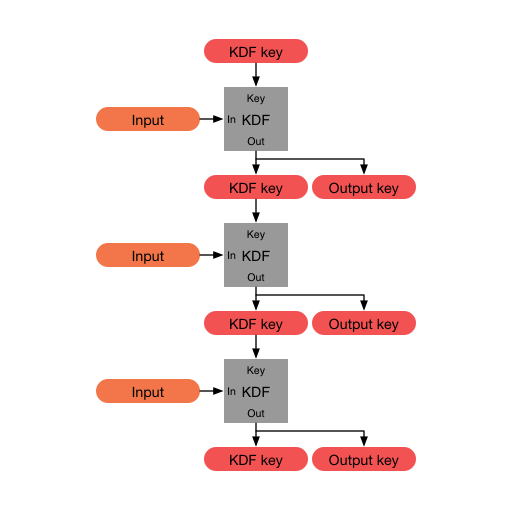
\includegraphics[width=0.5\textwidth]{figures/Signal_KDF_Chain.png}
    \caption{Showing flow of the key-derivation function itself (grey blocks) and its output-data (KDF key and output key) between ephemeral-triggers (sending a new message, in this context). The `ratchet' is, in effect, then advanced for next KDF. Public domain image; see \cite{signal:double_ratchet} for origin.} %TODO check wording here
    \label{fig:signal_kdf_chain}
\end{figure}
\subparagraph{Symmetric-Key Ratchet}
\label{subpara:symmetric-key_ratchet}
\noindent\\
This is where the (single) ratchet aspect comes in -- ratchet referring to how a mechanical ratchet's allowed-movement is unidirectional, but also in this context the data changing per ratchet step, such that the output key can be different per message, still based on the original shared secret (forming the root chain) (optionally) shared via PQ methods such as (the aforementioned lattice-based approach), Kyber forming part of PQXDH. This method works if only the key is somehow discovered for a single message, however as the chain key has not been stolen, all previous, and future, messages cannot be decrypted in the event one message's key is compromised, and this is the basis for forward secrecy, since the compromised key is only relevant for the message encrypted with the current `link' in the KDF chain, as such unless the KDF chain is compromised, the singe compromised key cannot be used for past/future messages.\\
However, despite the above attempting to gain forward secrecy by using a symmetric-key ratchet, using this alone cannot guarantee forward secrecy, since if the sending and receiving KDF chain keys are compromised -- this would allow all future messages to be decrypted, since to allow messages that arrive out-of-order, added to the message header when sending a message is the number of the current `link' in the KDF chain, whose key was thence used in encrypting the current message -- such header information would allow an attacker, having compromised a KDF sending and receiving chain, to know which message corresponds to which ratchet-step, and in turn, which key to use in decryption\footnote{It is worth noting that the header itself, containing the message's link in the KDF chain identifier can be encrypted, this is, however, mainly to prevent identification of ordering of messages (potentially-useful metadata), as well as preventing an eavesdropper determining which messages are sent to which contact (even if their name is unknown), this may also present itself as potentially-revealing metadata. For further reading on this, please see \textcolor{red}{link led from} \cite{signal:double_ratchet}}. Whilst this additional header information does allow the receiver to calculate keys ahead of the present link in their receiving KDF chain (to allow for messages which arrive out-of-order, as aforementioned), this would also allow an attacker to read all future messages, \textcolor{red}{and if all existing links in KDF chain were compromised (stored on-device (for as long as message exists, i.e. disappearing messages prevent long-term storage) -- much-less likely), this would also allow past messages to be decrypted} \citep{signal:double_ratchet}.\\%TODO fact-check this! && if need that citation here
\subparagraph{DH-Key Ratchet}
\label{subpara:dh-key_ratchet}
\noindent\\
Henceforth, an additional ratchet is used: Diffie-Hellman- key(s) ratchet -- this works by updating chain-keys based on Diffie-Hellman (DH) outputs (see \cref{para:diffie-hellman_primer}), rather than relying only on the symmetric-key ratchet (solving the issue if one party's sending and receiving chain keys are compromised, as mentioned above).\\
Updating the chain-keys from DH outputs is implemented by each party generating a DH- key-pair, then, at this starting point of this KDF chain, each has their own ratchet key-pair. Now one party, e.g. Bob, sends his starting ratchet-step public key from his starting key-pair to Alice, Alice now `combines' (see \cref{para:diffie-hellman_primer}) Bob's public key with her starting private key, as such she now has a new key-pair, partly based off Bob's starting public key. Now, still part of initialisation, Alice sends her new key-pair's public key to Bob, who thence performs a ratchet step, similarly to Alice, i.e. combining her public key with his starting private key. When a sender sends a message, they include their current ratchet step public key in the message header, upon the receiver receiving the message, and, by extension, receiving a new ratchet- public-key, the receiver performs a DH ratchet step, wherein the receiver uses the received public key, from the received-message's header, to replace their current ratchet- key-pair with a new key-pair, this process occurs by combining the received public key with the local party's (receiver) private key from their existing DH- key-pair, in this way, a sent message advertises the sender's public key for the current ratchet step. For example, with reference to \cref{fig:signal_message_dh_ratchet_step}, when Alice receives a message (initialisation now completed) she uses the received public key to perform a DH ratchet step (visible in \cref{fig:signal_message_dh_ratchet_step} where the public key from Alice is pointing to Bob's public key, since this DH output is performed using his public key), thereby `replacing her ratchet key-pair (observable in the first DH output under the blue line, also shown as equal to Bob's DH output at that point in the ratchet), deriving two DH outputs, one which matches Bob's latest [DH output] (as just mentioned), and a new one' \textcolor{red}{(for a potential outgoing message from Alice, with her latest key-pair shown in the furthest- bottom-left of the figure)} \citep{signal:double_ratchet}. %TODO fact check if btm-left keypair for outgoing...?
\begin{figure}[h!]
    \centering
    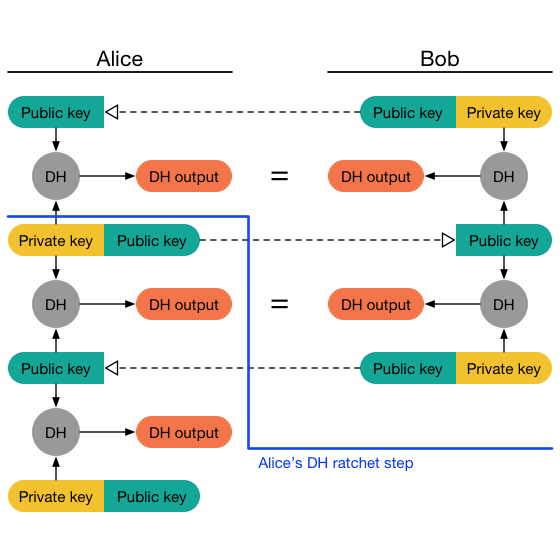
\includegraphics[width=0.5\textwidth]{figures/Signal_Message_DH_Ratchet_Step.png}
    \caption{The first DH ratchet step once, in this example, Alice has received the first message from Bob, showing how a ratchet step is performed (all that which is below the blue line), for a message, post-initialisation. Public domain image; see \cite{signal:double_ratchet} for origin.} %TODO check wording here
    \label{fig:signal_message_dh_ratchet_step}
\end{figure}
\begin{figure}[h!]
    \centering
    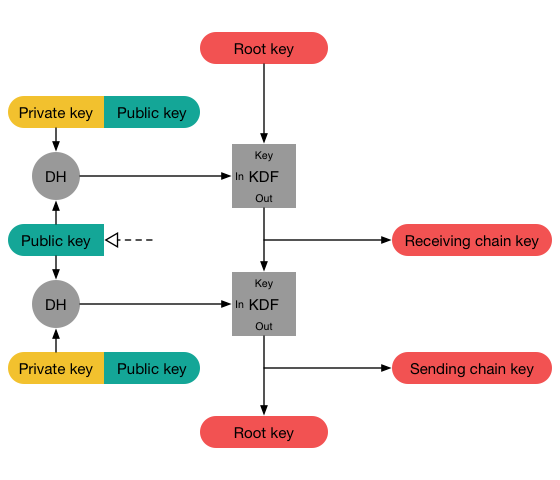
\includegraphics[width=0.5\textwidth]{figures/Signal_DH_Ratchet_Outputting_to_KDF_Chains.png}
    \caption{Full DH ratchet step, showing a double DH output (per full ratchet step), the top one to match the other party's, and a new key pair then sending a message, each fed into a separate KDF, each then deriving a sending and a receiving chain. Public domain image; see \cite{signal:double_ratchet} for origin.} %TODO check wording here+fact check
    \label{fig:signal_dh_ratchet_with_kdf_chains}
\end{figure}
However, a full DH ratchet step does not use solely the DH output (as observable in \cref{fig:signal_dh_ratchet_with_kdf_chains}), instead a DH output is the input to a KDF (which then derives either the receiving or sending chain key), this input takes the place of the unlabelled `input' to the KDFs seen in \cref{fig:signal_kdf_chain}. In \cref{fig:signal_dh_ratchet_with_kdf_chains}, observable is the aforementioned double DH output, the first to match the other party's DH output, but this is then fed into a KDF to improve `resilience and break-in recovery' \citep{signal:double_ratchet}, and the second DH output, as input to the second KDF, is to then derive a sending chain key, taking the place of the previous second DH output per full DH ratchet step.
\subparagraph{Double Ratchet}
\noindent\\
Combining both the symmetric-key ratchet and the DH-key ratchet produces the Double-Ratchet Algorithm (DRA). Given that public keys are sent in a message's header, when a party receives a new ratchet public key, they perform a full DH ratchet step, thereby replacing both chain keys (sending and receiving) -- this is the DH-key ratchet. After the DH-key ratchet, when a message is sent, a symmetric-key ratchet step occurs to the sending chain, thereby deriving the message key; similarly, when a message is received, the receiver performs a symmetric-key ratchet step for their receiving chain -- this is the symmetric-key ratchet.
%TODO include: \textcolor{red}{so each message using the preesnt kdf output of the is the encryhpt for the sender chain or present link in chain is the decrypt key for the receiver which would their the same link in their receiver chain -- almost still asymmetric in the sense that use 1 chain for encrypt and other for decrypt but actuallly its still sytmmetyric because u have the receivers sending key because it's your receier chain link. anyway because each chain is derived from the root chain (sent via Kyber), well thisis the way in which Kyber is used as a KEM to distribute a shared secret forming the root chain which in turn forms each send/receive chain, this is verymuch beneficial, since have forward secrecy in that if one chain link key is exposed, cannot get next (do not have other Key? or rand data?)} %TODO check: is this right?+transpile
\citep{signal:double_ratchet}
%but also cannot get any other messages before it since the key differs with each link
